
\chapter{Subrutinas Fructuosas}
\label{fruitchap}

La mayoría de funciones de Perl que hemos usado, tales como
la funciones matemáticas, producen valores de retorno. Aún así,
la mayoría de funciones que hemos escrito hasta ahora son funciones
void: ellas tienen un efecto, como imprimir un valor,
pero no tienen un valor de retorno. En este capítulo, aprenderás
a escribir funciones fructuosas.

\section{Valores de Retorno}
\index{return!value}

Al llamar una función fructuosa de genera un valor de retorno,
el cual usualmente asignamos a una variable o usamos como 
parte de una expresión:

\begin{lstlisting}
my $pi = 4 * atan 1;
my $altura = $radio * sin $radianes;
\end{lstlisting}
%
Muchas de las subrutinas que hemos escrito hasta ahora son
void. Hablando casualmente, ellas no tienen un valor de 
retorno útil; más precisamente, su valor de retorno puede
ser {\tt Any}, {\tt Nil}, {\tt ()}, o {\tt True}.

En este capítulo, finalmente escribiremos subrutinas fructuosas. 
El primer ejemplo es {\tt area}, la cual devuelve el área de un 
círculo con un radio en particular:

\begin{lstlisting}
sub area($radio) {
    my $area_circular = pi * $radio**2;
    return $area_circular;
}
\end{lstlisting}
%
Hemos visto la sentencia {\tt return} anteriormente,
pero en una subrutina fructuosa la sentencia {\tt return} 
incluye una expresión. Esta sentencia quiere decir: ``
Devuelve inmediatamente desde esta función y usa la siguiente
expresión como un valor de retorno.``
La expresión puede ser arbitrariamente complicada, así podríamos
esta función en una manera más concisa:
\index{return!statement}
\index{statement!return}

\begin{lstlisting}
sub area($radio) {
    return pi * $radio**2;
}
\end{lstlisting}
%

Por otro lado, las {\bf variables temporales} 
como \verb|area_circular| hace la depuración mucho más
fácil. También ayudar a documentar lo que está sucediendo
en la función.
\index{temporary variable}
\index{variable!temporary}

Algunas veces es útil tener varias sentencias return, por 
ejemplo una en cada rama de una condicional:

\begin{lstlisting}
sub valor_absoluto($num){
    if $num < 0 {
        return -$num;
    } else {
        return $num;
    }
}
\end{lstlisting}
%
Dado que estas sentencias {\tt return} están en una 
condicional alternativa, solo una se ejecuta.

Esto podría también escribirse de forma concisa usando sintaxis 
del modificador de sentencia:

\begin{lstlisting}
sub valor_absoluto($num){
    return -$num if $num < 0;
    return $num;
}
\end{lstlisting}
%
Otra vez, solo una de las sentencias return se ejecuta: si el 
número es negativo, la primera sentencia return es ejecutada
y la ejecución de la subrutina termina ahí; en cambio, si el
número es positivo o cero, solo la segunda sentencia return 
es ejecutada.

Tan pronto una sentencia return es ejecutada, la función termina
sin ejecutar las sentencias subsecuentes. Cualquier código que aparece
después de una sentencia {\tt return} incondicional, o cualquier
otro lugar que el flujo de ejecución no puede alcanzar es 
conocido como {\bf código muerto}. 
\index{dead code}

En una función fructuosa, es buena idea asegurar que cada
posible ruta a través del programa alcance con una sentencia
{\tt return}. Por ejemplo:

\begin{lstlisting}
# ADVERTENCIA: código con fallas
sub valor_absoluto($num){
    if $num < 0 {
        return -$num;
    } 
    if $num > 0 {
        return $num;
    }
}
\end{lstlisting}
%

Esta subrutina es incorrecta porque si {\tt \$num} es 0, 
ninguna de las condiciones es verdadera, y la subrutina termina 
sin alcanzar una sentencia {\tt return}. Si el flujo de ejecución
llega al final de una función, el valor de retorno es {\tt ()}, que básicamente
significa ``no definido`` y claramente no es el valor absoluto de 0:
\index{undefined value}

\begin{lstlisting}
> valor_absoluto(0)
()
\end{lstlisting}
%
Casualmente, Perl provee una función integrada
llamada {\tt abs} que calcula valores absolutos.
\index{abs function or method}
\index{function!abs}

\label{compare}
Como ejercicio, escribe una subrutina {\tt comparar}
que toma dos números, {\tt \$x} y {\tt \$y}, y devuelve
{\tt 1} si {\tt \$x > \$y}, {\tt 0} if {\tt \$x == \$y}, y 
{\tt -1} if {\tt \$x < \$y}.

Solución: \ref{sol_compare}
\index{compare function}
\index{function!compare}


\section{Desarrollo Incremental}
\label{incremental.development}
\index{development plan!incremental}
\index{incremental development}

A medida que escribes funciones más largas, puedes 
pasar más tiempo depurando.

Para tratar con programas complejos, podrías querer 
usar un proceso llamado {\bf desarrollo incremental}. El 
objetivo del desarrollo incremental es evitar sesiones largas\
y tediosas de depuración al añadir y evaluar una pequeña pieza
de código a la vez.
\index{testing!incremental development}
\index{Pythagorean theorem}

Como un ejemplo, supón que quieres encontrar la distancia 
entre dos puntos, dadas las coordenadas cartesianas o rectangulares
$(x_1, y_1)$ y $(x_2, y_2)$ de los puntos. Por el teorema de Pitágoras,
la distancia es:
\index{Pythagorean theorem}
\index{Cartesian coordinates}
\index{coordinates!Cartesian}
\index{rectangular!coordinates}
\index{coordinates!rectangular}


\begin{displaymath}
\mathrm{distancia} = \sqrt{(x_2 - x_1)^2 + (y_2 - y_1)^2}
\end{displaymath}
%
El primer paso es considerar cómo la función {\\t distancia} 
debería lucir en Perl. En otras palabra,cuáles son las entradas (parámetros)
y cuál es la salida (valor de retorno)?

En este caso, las entradas son los puntos, los cuales puedes 
representar usando cuatros números. El valor de retorno es la distancia
representada por un valor numérico.

Inmediatamente puedes escribir un bosquejo de la función:

\begin{lstlisting}
sub distancia($x1, $y1, $x2, $y2) {
    return 0.0;
}
\end{lstlisting}
%
Obviamente, esta versión no calcula la distancia; siempre 
devuelve cero. Sin embargo, es sintácticamente correcta, y 
puede ser ejecutada, lo que significa que la probaste antes 
de hacerla más complicada.

Para probar la nueva función, llámala con algunos argumentos:

\begin{lstlisting}
> distancia(1, 2, 4, 6);
0.0
\end{lstlisting}
%
Elegí estos valores para que la distancia horizontal sea 3 y la distancia
vertical seaa 4; de esa manera, el resultado es 5, la hipotenusa de 
un triángulo 3-4-5. Al probar una función, es siempre útil saber la 
respuesta correcta.
\index{testing!knowing the answer}

En este momento, hemos confirmado que la función es sintácticamente 
correcta, y podemos comenzar a añadir código al cuerpo de
la función. Un siguiente paso razonable es encontrar las diferencias
$x_2 - x_1$ and $y_2 - y_1$.  La siguiente versión almacena esos valores
en variable temporales y los imprime:

\begin{lstlisting}
sub distancia($x1, $y1, $x2, $y2) {
    my $dx = $x2 - $x1;
    my $dy = $y2 - $y1;
    say '$dx es', $dx;
    say '$dy es', $dy;
    return 0.0;
}
\end{lstlisting}
%
Si la subrutina funciona como debe, debería mostrar \verb"$dx es 3" y 
\verb"$dy es 4" (y todavía devolver 0.0). Si esto sucede, sabemos
que la función está recibiendo los argumentos correctos y realizando
la primera computación correctamente. Por lo contrario, si esto no sucede
solo tenemos que depurar algunas líneas.

El siguiente paso es computar la suma de los cuadrados de {\tt \$dx} y 
{\tt \$dy}:

\begin{lstlisting}
sub distancia($x1, $y1, $x2, $y2) {
    my $dx = $x2 - $x1;
    my $dy = $y2 - $y1;
    my $dist-cuadrada = $dx**2 + $dy**2;
    say '$dist-cuadrada es: ', $dist-cuadrada;
    return 0.0;
}
\end{lstlisting}
%
Otra vez, ejecutarías el programa en esta etapa y 
chequearías la salida (que debería ser 25).
Finalmente, puedes usar la función integrada {\tt sqrt} 
para calcular la raíz cuadrada y devolver el resultado:
\index{sqrt function}
\index{function!sqrt}

\begin{lstlisting}
sub distancia($x1, $y1, $x2, $y2) {
    my $dx = $x2 - $x1;
    my $dy = $y2 - $y1;
    my $dist-cuadrada = $dx**2 + $dy**2;
    my $resultado = sqrt $dist-cuadrada;
    return $resultado;
}
\end{lstlisting}
%
Si eso funciona correctamente, ya acabaste. Por lo contrario,
podrías imprimir el valor de {\tt \$resultado} antes de la
sentencia return.

La versión final de la subrutina no muestra nada cuando se ejecuta;
solo devuelve un valor. Las sentencias {\tt print} que escribimos
son útiles para la depuración, pero una vez que consigues que la subrutina
funcione correctamente, puedes removerlas. Código como ese es algunas
veces llamado {\tt andamiaje} porque es útil para construir el programa
pero no forma parte del producto final.
\index{scaffolding}

Cuando empiezas a programar, debes agregar una o dos líneas de código
al mismo tiempo. A medida que ganas experiencia, puedes entonces escribir
y depurar piezas más grandes. De cualquier manera, el desarrollo incremental
puede salvarte muchas horas de depuración.

Los aspectos claves del proceso son:
\begin{enumerate}

\item Comienza con un programa que funcione y haz pequeños cambios
incrementales. En cualquier punto, si hay un error, deberías entonces
tener una buena idea donde se encuentra.

\item Usa variables para almacenar los valores intermedios
para que puedas mostrarlos y chequearlos

\item Una vez que el programa funciona, podrías querer remover
algo del código de andamiaje o consolidar sentencia múltiples
en una expresión compuesta, pero solo si no dificulta la lectura
del programa.

\end{enumerate}

Nota que, por lo menos para casos relativamente simples, 
puedes usar el REPL para probar expresiones y hasta sentencias
multilíneas o subrutinas en el modo interactivo antes de 
incluirlas en tu código. Esto es usualmente rápido y puede 
ahorrarte algún tiempo.
\index{REPL}
\index{interactive mode}

\label{hypotenuse}
Como ejercicio, usa el desarrollo incremental para escribir
una función llamada {\tt hipotenusa} que devuelve la longitud de
la hipotenusa de un triángulo rectángulo, dadas las longitudes de
los otros dos lados como argumentos. Registra cada etapa del
desarrollo a medida que avanzas.

Solución: \ref{sol_hypotenuse}.
\index{hypotenuse}



\section{Composición}
\index{composition}
\index{function composition}

Como deberías saber por ahora, tú puedes llamar una función
desde otra. Como un ejemplo, escribiremos una función 
que toma dos puntos, el centro del círculo y un punto en el 
perímetro, y calcula el área del círculo.

Asume que el centro es almacenado en las variables {\tt \$x-c} y
{\tt \$y-c}, y el perímetro está en {\tt \$x-p} y {\tt \$y-p}. 
El primer paso es encontrar el radio del círculo, el cual es la 
distancia entre los dos puntos. Anteriormente escribimos una función,
{\tt distancia}, que hace exactamente eso:

\begin{lstlisting}
my $radio = distancia($x-c, $y-c, $x-p, $y-p);
\end{lstlisting}
%
El siguiente paso es encontrar el área de un círculo 
con ese radio; también escribimos algo para hacer eso mismo:

\begin{lstlisting}
my $resultado = area($radio);
\end{lstlisting}
%
Al encapsular estos pasos en una función, tenemos:
\index{encapsulation}

\begin{lstlisting}
sub area-círculo($x-c, $y-c, $x-p, $y-p) {
    my $radio = distancia($x-c, $y-c, $x-p, $y-p);
    my $resultado = area($radio)
    return $resultado;
}
\end{lstlisting}
%
Las variables temporarias {\tt \$radio} y {\tt \$resultado} son útiles
para el desarrollo y la depuración, pero una vez que el programa ya funciona
adecuadamente, podemos hacer todo más conciso al componer las llamadas
de las funciones:

\begin{lstlisting}
sub area-círculo($x-c, $y-c, $x-p, $y-p) {
    return area distancia($x-c, $y-c, $x-p, $y-p);
}
\end{lstlisting}
%

La última línea del ejemplo anterior ahora funciona como
un conducto (del inglés \emph{pipeline}) de datos desde la 
derecha hacia la izquierda; la función \verb|distancia| toma 
los cuatros argumentos y devuelve una distancia (el radio)
el cual se pasa como una argumento a \verb|area|; con este
argumento, \verb|area| es ahora capaz de devolver el área,
la cual es entonces devuelta por \verb|area-círculo| al
código que hace la llamada. Regresaremos más tarde a este modelo
de conducto de datos.
\index{pipe-line programming}

\section{Funciones Booleanas}
\label{boolean}

Las funciones pueden devolver valores Booleanos, lo cual es usualmente
conveniente para ocultar pruebas complicadas dentro de las funciones. Por
ejemplo:
\index{Boolean function} 

\begin{lstlisting}
sub es-divisible(Int $x, Int $y) {
    if $x % $y == 0 {
        return True;
    } else {
        return False;
    }
}
\end{lstlisting}
%
Es común darle a las funciones Booleanas nombres que suenan como
preguntas con respuestas de sí/no; \verb|es-divisible|, por ejemplo,
devuelve {\tt True} o {\tt False} para indicar si {\tt x} es divisible
por {\tt y}.

Este es un ejemplo:

\begin{lstlisting}
> es-divisible(6, 4);
False
> es-divisible(6, 3);
True
\end{lstlisting}
%
El resultado del operador {\tt ==} es un valor Booleano,
así que podemos escribir la subrutina de manera concisa al 
devolverlo directamente:

\begin{lstlisting}
sub es-divisible(Int $x, Int $y) {
    return $x % $y == 0
}
\end{lstlisting}
%
Si no hay una sentencia de retorno, una subrutina en Perl devuelve
el valor de la expresión en la última línea de código de la 
subrutina (provisto que la última expresión sea una expresión
que puede ser evaluada), así que la sentencia {\tt return} no 
es requerida aquí. Además, dado que 0 es una valor falso y cualquier 
otro entero es un valor verdadero, la misma subrutina podría escribirse
de otra forma:

\begin{lstlisting}
sub es-divisible(Int $x, Int $y) { 
    not $x % $y 
}
\end{lstlisting}

Las declaraciones de tipo {\tt Int} en las signaturas de la subrutina
más arriba no son necesarias. La subrutina funcionaría sin ellas, pero
ellas pueden proveer algún tipo de protección en contra del uso 
de esta subrutina con argumentos defectuosos.

Las funciones Booleanas se usan usualmente en los 
modificadores de sentencias:
\index{statement modifier}
\index{modifier!statement}

\begin{lstlisting}
say "$x es divisible por $y" if es-divisible($x, $y);
\end{lstlisting}
%
Podría ser tentativo escribir algo como:

\begin{lstlisting}
say "$x es divisible por $y" if es-divisible($x, $y) == True;
\end{lstlisting}
%
Pero la comparación extra no es necesaria: 
{\tt es-divisible} devuelve un valor Booleano que puede ser
interpretado directamente por la condicional {\tt if}.

\label{isbetween}
Como ejercicio, escribe una función \verb|está-entre(x, y, z)|
que devuelve {\tt True} si $x \le y \le z$ o por lo contrario,
{\tt False}.

Solución: \ref{sol_isbetween}.

\section{Un Lenguaje de Programación Completo}

En la sección anterior vimos varias maneras de escribir
una subrutina para chequear la divisibilidad de dos 
enteros.
\index{divisibility}

De hecho, como fue mencionado anteriormente, Perl~6
tiene un operador ``es-divisible``, \verb|%%|, el cual
devuelve {\tt True} si el número en la izquierda es divisible
por el de la derecha:
%\index{%%!is divisible operator}
\index{is divisible operator}

\begin{lstlisting}
> 9 %% 3
True
> 9 %% 4
False
\end{lstlisting}

Por lo tanto no había necesidad de escribir la subrutina
{\tt es-divisible}. Pero no te preocupes, es totalmente 
normal si no recordaste eso. A los hablantes de lenguajes 
naturales se les permite tener diferentes niveles de cualificación,
aprender a medida que avanzan, y poner el lenguaje a buen uso 
antes de que sepan el lenguaje completo. Lo mismo pasa con Perl.
Tú (y yo) no sabemos todo sobre Perl~6 todavía, al igual que no
sabemos todo sobre el inglés (o el español). Pero es de hecho 
``Oficialmente Okay en la Cultura de Perl`` usar el subconjunto
del lenguaje que sabes. De hecho, se fomenta a que uses lo que es
a veces llamado ``baby Perl`` para escribir programas, aunque sean
un poco toscos y rudimentarios al principio. Esa es la mejor manera 
de aprender Perl, del mismo que ``hablar como un bebé`` (``baby talk``) es
la mejor manera para que un niño aprenda inglés (o español).
\index{baby Perl}
\index{Perl culture}

El número de maneras diferentes de llevar a cabo una tarea,
tal como chequear si un número es divisible por otro,
es un ejemplo del lema de Perl:
\emph{there is more than one way to do it 
(Hay más de una forma para hacer algo)}, usualmente abreviado TIMTOWTDI.
Algunas maneras pueden ser más concisa o más eficiente que
otras, pero, en la filosofía de Perl, tú estás perfectamente 
facultado para hacerlo a tu manera, especialmente si eres
un principiante, provisto que encuentres el resultado 
correcto.
\index{there is more than one way to do it}
\index{TIMTOWTDI}
\index{Turing!complete language}
\index{language!Turing complete}
\index{Turing, Alan}
\index{Turing!thesis}

Hasta ahora, solamente hemos cubierto un pequeño subconjunto de Perl~6,
pero te sería interesante saber que este subconjunto es un lenguaje
de programación \emph{completo}, lo cual significa que esencialmente
cualquier cosa que puede computarse podría expresarse en este 
lenguaje. Cualquier programa que se haya escrito jamás podría escribirse
de nuevo solo usando las características del lenguaje que has aprendido
hasta ahora (actualmente, solo necesitarías algunos comandos para
controlar dispositivos como el ratón, discos, redes, etc., pero eso 
es todo).

La prueba de esa afirmación no es un ejercicio trivio. El primero
en probarla fue Alan Turing, uno de los primeros científicos de la
computación (algunas personas argumentan que él fue un matemático, sin 
embargo muchos de los primeros científicos de la computación comenzaron 
como matemáticos). Por esta razón, se le conoce como la prueba de Turing
(\emph{Turing Test}). Para una discusión más completa (y precisa) de la
prueba de Turing, recomiendo el libro  {\em Introduction to the
Theory of Computation} de Michael Sipser.

\section{Más Recursión}
\label{more.recursion}
\index{recursion}


Para darte una idea de lo que puedes hacer con las herramientas
que has aprendido hasta ahora, evaluaremos algunas funciones 
matemáticas definidas de forma recursiva. Una definición recursiva
es similar a una definición circular, en el sentido de que la 
definición contiene una referencia a la cosa que se define. 
Una definición verdaderamente circular no es muy útil:

\begin{description}

\item[Vorpal] An adjective used to describe something that is vorpal.
\index{vorpal}
\index{circular definition}
\index{definition!circular}

\end{description}

Si ves esa definición en el diccionario, podrías enojarte. 
Sin embargo, si busca la definición de la función factorial,
denotada con el símbolo $!$, podrías conseguir algo como esto:
%
\begin{eqnarray*}
&&  0! = 1 \\
&&  n! = n (n-1)!
\end{eqnarray*}
%
Esta definición dice que el factorial de 0 es 1, y que el factorial
de cualquier otro valor (entero positivo), $n$, es 
$n$ multiplicado por el factorial de $n-1$.

Así que $3!$ es 3 por $2!$, el cual es 2 por $1!$, el cual es 1 por
$0!$. Si lo ponemos todo junto, $3!$ es igual a 3 por 2 por 1 por 1, 
lo cual es 6.
\index{factorial!function}
\index{function!factorial}
\index{recursive definition}

Si puedes escribir una definición recursiva de algo, puedes escribir
un programa de Perl para evaluar dicha definición. El primer paso
es decidir cuáles deberían ser los parámetros. En este caso, es
claro que el factorial toma un número\footnote{Debería ser realmente un entero, pero regresaremos a esto más tarde en este capítulo.}:

\begin{lstlisting}
sub factorial($n){
}
\end{lstlisting}
%
Si el argumento es 0, todo lo que tenemos que hacer es devolver es 1:

\begin{lstlisting}
sub factorial($n){
    if $n == 0 {
        return 1;
    }
}   
\end{lstlisting}
%
Por el otro lado, y ésta es la parte interesante, tenemos que hacer
una llamada recursiva para encontrar el factorial de $n-1$ y después
multiplicarlo por $n$:
\index{factorial!using recursion}

\begin{lstlisting}
sub factorial($n){
    if $n == 0 {
        return 1;
    } else {
        my $recurse = factorial($n-1);
        my $result = $n * $recurse;
        return $result;
    }
}
\end{lstlisting}
%
El flujo de ejecución para este programa es similar al flujo de 
{\tt cuenta-regresiva} en la Sección~\ref{recursion}. Si llamamos
a {\tt factorial} con el valor 3:

Dado que 3 no es 0, tomamos la segunda rama y calculamos el factorial de
{\tt \$n-1}...

\begin{quote}
Dado que 2 no es 0, tomamos la segunda rama y calculamos el factorial de
{\tt \$n-1}...


  \begin{quote}
  Dado que 1 no es 0, tomamos la segunda rama y calculamos el factorial de
  {\tt \$n-1}...


    \begin{quote}
    Dado que 0 es igual a 0, tomamos la primera rama y devolvemos 1
    sin hacer más llamadas recursivas.
    \end{quote}

	
  El valor de retorno, 1, es multiplicado por \verb|$n|, el cual es 1,
  y se devuelve el resultado.
  \end{quote}


El valor de retorno, 1, es multiplicado por \verb|$n|, el cual es 1,
y se devuelve el resultado.
\end{quote}


El valor de retorno, 2, es multiplicado por \verb|$n|, el cual es 3,
el resultado, 6, se convierte en el valor de retorno de la llamada
de subrutina que inició todo el proceso.
\index{stack diagram}

La figura~\ref{fig.stack3} muestra como el diagrama de pila luce para esta
secuencia de llamadas de función.

\begin{figure}
\centerline
{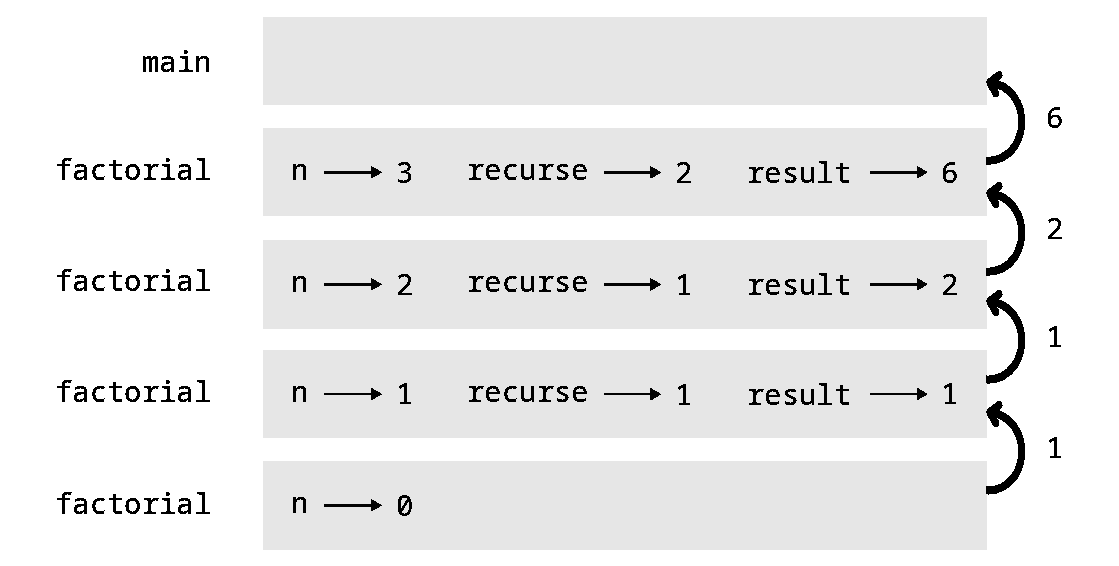
\includegraphics[scale=0.7]{figs/stack3.pdf}}
\caption{Diagrama de pila.}
\label{fig.stack3}
\end{figure}

Los valores de retorno se muestran siendo pasados devuelta a la pila. En cada
cuadro, el valor de retorno es el valor de {\tt result}, el cual es 
producto de {\tt n} y {\tt recurse}.
\index{function!frame}
\index{frame}

En el último cuadro, las variables locales {\tt recurse} y {\tt result}
no existen, porque la rama que las crea no se ejecuta.

Un programador de Perl con experiencia podría escribir una
subrutina más concisa o más idiomática\footnote{Luego veremos 
más formas idiomáticas de computar el factorial de un número.}:
\index{idiomatic}

\begin{lstlisting}
sub factorial($n){
    return 1 if $n == 0;
    return $n * factorial $n-1;
}
\end{lstlisting}
%
Esto es no mejor que nuestra primera versión, y probablemente
no se ejecutará significativamente más rápido, pero es presumiblemente
más clara, por lo menos cuando te acostumbra a este tipo de sintaxis.

\section{Acto de Fe}
\index{recursion}
\index{leap of faith}

Seguir el flujo de ejecución es una manera de leer un programa,
pero se vuelve agobiante en poco tiempo. Una alternativa es 
lo que puede ser llamada el ``acto de fe``. Cuando encuentras 
una subrutina, en lugar de seguir el flujo de ejecución,
tu \emph{asumes} que la subrutina funcione correctamente y devuelve
el resultado correcto.


De hecho, estás ya practicando este acto de fe cuando usas las funciones
integradas. Cuando llamas las funciones matemáticas tales como {\tt cos} 
o {\tt sqrt}, no examinas los cuerpos de esas funciones. Asumes que funcionan
adecuadamente porque las personas que escribieron las funciones 
integradas eran probablemente buenos programadores (y porque puedes
asumir seguramente que dichas funciones han sido probadas extensivamente).

Lo mismo es cierto cuando llamas una de tus subrutinas. Por ejemplo,
en la Sección~\ref{boolean}, escribimos una subrutina llamada \verb|es-divisible|
que determina si un número es divisible por otro. Una vez que nos convencimos
que esta subrutina es correcta---al examinar y probar el código---podemos
usar la subrutina sin mirar al cuerpo otra vez.
\index{testing!leap of faith}

Lo mismo es cierto para programas recursivos. Cuando obtienes la
llamada recursiva, en lugar de seguir el flujo de ejecución, deberías
asumir que la llamada recursiva funciona (devuelve el resultado correcto)
y después preguntarte, ``Asumiendo que puedo encontrar el factorial de
\verb|$n-1|, puedo yo calcular el factorial de \verb|$n|?`` Es bien claro 
que puedes, al multiplicar po \verb|$n|.

!`Por supuesto, es un poco extraño asumir que la subrutina funciona correctamente
cuando no has terminado de escribirla, pero por eso es que se conoce 
como un acto de fe!


\section{Otro Ejemplo Más}
\label{one.more.example}

\index{Fibonacci!function}
\index{function!Fibonacci}
Después de {\tt factorial}, el ejemplo más común de una función
matemática definida recursivamente es {\tt fibonacci}, la cual tiene
la siguiente definición (ver
  \url{https://es.wikipedia.org/wiki/Sucesión_de_Fibonacci}):
%
\begin{eqnarray*}
&& \mathrm{fibonacci}(0) = 1 \\
&& \mathrm{fibonacci}(1) = 1 \\
&& \mathrm{fibonacci}(n) = \mathrm{fibonacci}(n-1) + \mathrm{fibonacci}(n-2)
\end{eqnarray*}
%

En lenguaje llano, una sucesión de Fibonacci es una secuencia de
números tales como:
\begin{lstlisting}
1, 1, 2, 3, 5, 8, 13, 21, ...
\end{lstlisting}
donde los dos primeros términos son iguales a 1 y cualquier otro
término es la suma de los dos números que lo preceden.

Discutimos la secuencia de Fibonacci brevemente en el Ejercicio~\ref{fibonacci}
del capítulo anterior y la implementamos con un bucle {\tt for}.

Ahora traduzcamos la definición recursiva en Perl. Así es como luce:

\begin{lstlisting}
sub fibonacci ($n) {
    return 1 if $n == 0 or $n == 1;
    return fibonacci($n-1) + fibonacci($n-2)
}
\end{lstlisting}
%
Si tratas de seguir el flujo de ejecución aquí, aún para valores
pequeños de \verb|$n|, tu cabeza va a explotar. Sin embargo, de acuerdo
al acto de fe, si asumimos que las llamadas recursivas funcionan correctamente,
entonces es claro que obtendrás el resultado correcto al añadirlo todo 
junto.
\index{flow of execution}


\section{Chequeo de Tipos}
\label{guardian}

?`Qué pasa si llamamos {\tt factorial} y pasamos a 1.5 como un argumento?
\index{type!checking}
\index{error checking}
\index{factorial!function}

Al parecer conseguimos una recursión infinita. ?`Cómo puede ser?
La subrutina tiene una caso base---cuando {\tt \$n == 0}. Pero 
si {\tt \$n} no es un entero, podemos {\em perder} el caso base 
y hacer la recursión por siempre. 
\index{infinite recursion}
\index{recursion!infinite}
\index{base case}

En la primera llamada recursiva, el valor de {\tt \$n} es 0.5.
En la siguiente, es -0.5. Desde ahí, se vuelve más pequeño 
(más negativo), pero nunca será 0.

Tenemos dos opciones. Podemos tratar de generalizar la función
{\tt factorial} para funcionar con números que no son enteros, o
podemos hacer que {\tt factorial} haga un chequeo de sus argumentos.
La primera opción es llamada la función gamma y está fuera del alcance 
de este libro. Por lo tanto, discutiremos la segunda opción.
\index{function!gamma}
\index{gamma function}

Ya hemos visto ejemplos de subrutinas que usan la signatura para 
verificar el tipo del argumento. Así que podemos añadir el tipo
{\tt Int} al parámetro en la signatura. Mientras hacemos esto,
también podemos asegurarnos de que el argumento sea positivo o cero:

\begin{lstlisting}
sub factorial(Int $n where $n >= 0){
    return 1 if $n == 0;
    return $n * factorial $n-1;
}
\end{lstlisting}
%
\index{constraint}
\index{trait}
El tipo {\tt Int} en la signatura chequea por números no enteros,
lo cual ya lo sabemos. La parte {\tt where \$n >= 0} es una restricción
de parámetro: si el parámetro es negativo, la subrutina debería
fallar. Técnicamente, la restricción se implementa aquí dentro de la
signatura usando una característica sintáctica llamada un \emph{rasgo}
(\emph{trait} en inglés), que es una propiedad impuesta sobre el parámetro
al tiempo de compilación. Si el argumento que se pasa a la función no
es un entero o si es negativo, el programa imprime un 
mensaje de error para indicar que algo malo pasó:

\begin{lstlisting}
> say factorial 1.5
Type check failed in binding $n; expected Int but got Rat
  in sub factorial at <unknown file> line 1
  in block <unit> at <unknown file> line 1

> say factorial -3
Constraint type check failed for parameter '$n'
> say factorial "Fred"
Type check failed in binding $n; expected Int but got Str
  in sub factorial at <unknown file> line 1
  in block <unit> at <unknown file> line 1
\end{lstlisting}
% 
Si eludimos ambos chequeos, sabemos que \verb|$n|
es un entero y que es positivo o cero, así que podemos 
probar que la recursión termina.


\index{subset!type}
\index{type subset}
Otra modo de lograr un resultado similar es definir tu propio
subconjunto de tipos integrados. Por ejemplo, puedes crear un
subconjunto {\tt Par-entero} de enteros y después usarlo más o 
menos como si fuera un tipo para declarar tus variables o asignarle
un tipo a tus parámetros de las subrutinas:

\begin{lstlisting}
subset Par-entero of Int where { $_ %% 2 } # o : … where { $_ % 2 == 0 }
# Par-entero puede ahora usarse como un tipo

my Par-entero $x = 2; # OK
my Par-entero $y = 3; # Error de discordancia de tipo
\end{lstlisting}

De igual manera, en el caso de la subrutina {\tt factorial},
podemos crear un subconjunto de enteros no negativos y usarlos
para chequear el parámetro que se pasa a la subrutina:

\begin{lstlisting}
subset Entero-no-neg of Int where { $_ >= 0}
# ...

sub factorial(Entero-no-neg $n){
    return 1 if $n == 0;
    return $n * factorial $n-1;
}
\end{lstlisting}
%
Si pasamos un número negativo a la subrutina, 
podemos obtener un error similar al anterior:

\begin{lstlisting}
Constraint type check failed for parameter '$n'...
\end{lstlisting}

\index{guardian pattern}
\index{pattern!guardian}
Este programa demuestra un patrón conocido como un {\bf guardián}.
La signatura actúa como un guardián, que protege el código de valores
que podrían causar un error. Los guardianes hacen posible probar la validez
del código.

\section{Sobrecargas}
\label{multisubs}
\index{multi!subroutine}

Es posible escribir múltiple versiones de una subrutina 
con el mismo nombre pero con signaturas diferentes, por ejemplo
una \emph{aridad} diferente (una palabra sofisticada para referirse
al número de argumentos) o diferentes tipos del argumentos, usando 
la palabra clave {\tt multi}. En este caso, el interpretador 
elegirá la versión de la subrutina cuyo signatura mejor coincide con
la lista de argumentos.
\index{arity}

Por ejemplo, podríamos escribir de nuevo la función factorial como
sigue:
\index{factorial!using multi subroutines}

\begin{lstlisting}
multi sub fact(0) { 1 };
multi sub fact(Int $n where $n > 0) {
    $n * fact $n - 1;
}
say fact 0;   # -> 1
say fact 10;  # -> 3628800
\end{lstlisting}

Aquí, no entramos en una recursión infinita porque, cuando
el parámetro que se pasa a {\tt fact} es 0, es la primera de la
versión de la subrutina que se llama y devuelve un valor entero (1),
y esto termina la recursión.

Similarmente, la función Fibonacci puede escribirse de nuevo
con sobrecargas:
\index{Fibonacci!function with multi subroutines}

\begin{lstlisting}
multi fibonacci(0) { 1 }
multi fibonacci(1) { 1 }
multi fibonacci(Int $n where $n > 1) { 
    fibonacci($n - 2) + fibonacci($n - 1) 
}
say fibonacci 10;  # -> 89
\end{lstlisting}

Muchas de las funciones integradas y muchos de los operadores de Perl~6 
son escritos como sobrecargas.

\section{Depuración de programas}
\label{factdebug}

La fragmentación un programa grande en funciones o subrutinas más
pequeñas crea puestos de control naturales para la depuración.
Si una subrutina no está funcionando, existen tres posibilidades
para considerar:
\index{debugging} 

\begin{itemize}

\item Hay algo incorrecto con los argumentos que la subrutina
recibe; una precondición es violada.

\item Hay algo incorrecto con la subrutina; una poscondición
es violada.

\item Hay algo incorrecto con el valor de retorno o la forma
en la cual es usado.

\end{itemize}

Para descartar la primera posibilidad, puedes agregar una
sentencia de impresión al inicio de la función y mostrar los valores
de los parámetros (y tal vez sus tipos). O puedes escribir 
código para chequear las precondiciones explícitamente.
\index{precondition}
\index{postcondition}

Para el propósito de depuración, es usualmente útil imprimir
el contenido de una variable o de un parámetro dentro de 
una cadena de texto con caracteres alrededor, para así 
visualizar caracteres que de otra manera son invisibles, tales
como espacios o caracteres de nueva línea. Por ejemplo, piensas
que la \verb|$var| debería contener ``two```y ejecutar la 
siguiente prueba:
\begin{lstlisting}
if $var eq "two" {
    do-something()
}
\end{lstlisting}
%
Pero falla y la subrutina {\tt do-something} nunca se ejecuta.

Quizás quieres usar una sentencia de impresión que 
corroborará el contenido de \verb|$var|:
\begin{lstlisting}
say "[$var]";
if $var eq "two" {
    do-something()
}
\end{lstlisting}
%

Esto podría imprimir:
\begin{lstlisting}
[two ]
\end{lstlisting}
%

o:
\begin{lstlisting}
[two
]
\end{lstlisting}
%
Ahora sabes que la prueba de igualdad falla porque 
\verb|$var| contiene un carácter colgante (espacio o nueva línea)
que podría ser difícil de detectar.

Si los parámetros están bien, agrega una sentencia {\tt print}
antes de cada sentencia {\tt return} y muestra el valor de retorno.
Si es posible, chequea el resultado manualmente. Considera llamar 
la función con valores que facilitan chequear el resultado
(como en la Sección~\ref{incremental.development}).

Si la función aparenta funcionar, observa la llamada de la función
para asegurarte que el valor de retorno está siendo utilizado 
correctamente (o apenas siendo utilizado).
\index{flow of execution}

Agregar sentencias de impresión al comienzo y final de una función
ayuda a hacer al flujo de ejecución más visible. 
Por ejemplo, la siguiente es una versión de {\tt factorial}
con sentencias de impresión:
\index{factorial!recursive function with debug statements}

\begin{lstlisting}
sub factorial(Int $n) {
    my $espacio = ' ' x (4 * $n);
    say $espacio, 'factorial ', $n;
    if $n == 0 {
        say $espacio, 'devolviendo 1';
        return 1;
    } else {
        my $result = $n * factorial $n-1;
        say $espacio, 'devolviendo ', $result;
        return $result;
    }
}
\end{lstlisting}
%
La variable {\tt \$espacio} es una cadena de caracteres de espacio que 
controla la indentación de la salida. Este es el resultado para 
{\tt factorial(4)}:

\begin{lstlisting}
                factorial 4
            factorial 3
        factorial 2
    factorial 1
factorial 0
devolviendo 1
    devolviendo 1
        devolviendo 2
            devolviendo 6
                devolviendo 24
\end{lstlisting}
%
Si estás confundido sobre el flujo de ejecución, este tipo
de salida puede ser útil. Toma tiempo desarrollar andamiaje 
efectivo, pero un poco de andamiaje puede ahorrar mucho 
tiempo de depuración.

\section{Glosario}

\begin{description}

\item[Variable temporal]  Una variable usada para almacenar un valor
intermedio en una operación compleja.
\index{temporary variable}
\index{variable!temporary}

\item[Código muerto]  Parte de un programa que nunca se ejecuta, usualmente
porque aparece después de una sentencia {\tt return}.
\index{dead code}

\item[Desarrollo incremental]  Un plan de desarrollo de programa 
destinado a evitar la depuración al añadir y probar solo piezas
pequeñas de código a la vez.
\index{incremental development}

\item[Andamiaje]  Código usado durante el desarrollo de un programa
pero que no es parte de la versión final.
\index{scaffolding}

\item[Guardián]  Un patrón de programación que usa una sentencia
condicional para chequear y manejar circunstancias que podría causar
un error.
\index{guardian pattern}
\index{pattern!guardian}

\end{description}


\section{Ejercicios}

\begin{exercise}

Dibuja un diagrama de pila para el siguiente programa.
?`Qué imprime el programa? Por favor trata de contestar estas
preguntas antes de ejecutar el programa.
\index{stack diagram}

\begin{lstlisting}
sub b(Int $z) {
    my $prod = a($z, $z);
    say $z, " ", $prod;
    return $prod;
}
sub a(Int $x is copy, Int $y) {
    $x++;
    return $x * $y;
}
sub c(Int $x, Int $y, Int $z) {
    my $total = $x + $y + $z;
    my $square = b($total) ** 2;
    return $square;
}

my $x = 1;
my $y = $x + 1;
say c($x, $y + 3, $x + $y);
\end{lstlisting}

\end{exercise}


\begin{exercise}
\label{ackermann}
\index{Ackermann function}

La función de Ackermann, $A(m, n)$, se define como sigue:

\begin{eqnarray*}
A(m, n) = \begin{cases} 
              n+1 & \mbox{if } m = 0 \\ 
        A(m-1, 1) & \mbox{if } m > 0 \mbox{ and } n = 0 \\ 
A(m-1, A(m, n-1)) & \mbox{if } m > 0 \mbox{ and } n > 0.
\end{cases} 
\end{eqnarray*}
%
Ver \url{https://es.wikipedia.org/wiki/Funci%C3%B3n_de_Ackermann}.
Escribe una subrutina llamada {\tt ack} que evalúa la función de Ackermann.
Usa tu subrutina para evaluar {\tt ack(3, 4)}, que debería ser 125. 
?`Qué pasa con valores más grandes de {\tt m} y {\tt n}?

Solución: \ref{sol_ackermann}.
\index{Ackermann function}
\index{function!ack}

\end{exercise}


\begin{exercise}
\label{palindrome}
\index{palindrome}

Un palíndromo es una palabra que que se lee igual adelante que atrás,
como ``Ana`` y ``radar``. Recursivamente, una palabra es un palíndromo
si las primera y últimas letras son las mismas y el medio es un palíndromo.
\index{palindrome}

La siguientes son subrutinas que toman un argumento de cadena de texto
y devuelve las letras primera, última y del centro:

\begin{lstlisting}
sub primera_letra(Str $palabra){
    return substr $palabra, 0, 1;
}

sub última_letra(Str $palabra){
    return substr $palabra, *-1, 1;
}

sub centro_letra(Str $palabra){
    return substr $palabra, 1, *-1;
}
\end{lstlisting}
%
Por el momento, no es necesario que sepas cómo funcionan; veremos esto en el 
Capítulo~\ref{strings} sobre cadenas de texto. Por ahora:

\begin{enumerate}

\item Escribe estas subrutinas en un archivo llamado 
{\tt palindromo.pl6} y pruébalas. ?`Qué pasas si llamas 
a \verb|letra_centro| con una cadena de texto con dos letras?
?`Una letra? ?`Qué pasa con una cadena de texto, la cual se escribe
\verb|''| y no contiene letras? Dado que el método {\tt .chars}
devuelve la longitud de una cadena de texto, cómo podrías añadir
una restricción de signatura para rechazar una entrada inválida?

\item Escribe una subrutina llamada \verb|es-palindromo| que toma
una cadena de texto como argumento y devuelve {\tt True} si es 
un palindromo y {\tt False} de lo contrario. Recuerdas que puedes
usar el método integrado {\tt .chars} para chequear la longitud 
de una cadena de texto.

\end{enumerate}

Solución: \ref{sol_palindrome}.
\index{palindrome}

\end{exercise}

\begin{exercise}
\index{power}
\label{power}

Un número entero. $a$, es una potencia de $b$ si es divisible 
por $b$ y $a/b$ es una potencia de $b$. Escribe una función llamada
\verb|es-potencia-de| que toma los parámetros {\tt a} y {\tt b}
y devuelve {\tt True} si {\tt a} es una potencia de {\tt b}.
Nota: tendrás que pensar sobre el caso base.
\index{base case}

Solución: \ref{sol_power}

\end{exercise}


\begin{exercise}
\index{greatest common divisor (GCD)}
\index{GCD (greatest common divisor)}
\label{gcd}
\index{gcd function}

El máximo común divisor (MCD) de $a$ y $b$ es el mayor número entero
que los divide sin dejar un residuo.

Una manera de encontrar el MCD de dos números está basada en la
observación de que si $r$ es el residuo cuando $a$ es dividido por $b$,
entonces $mcd(a,b) = mcd(b,r)$. Como un caso base, podemos usar 
$mcd(a, 0) = a$.

Escribe una función llamada \verb|mcd| que toma los parámetros 
{\tt a} y {\tt b} y devuelve su máximo común divisor.

Crédito: este ejercicio está basado en un ejemplo de 
{\em Structure and Interpretation of Computer Programs}
de Abelson y Sussman.
\index{Abelson, Harold}
\index{Sussman, Gerald Jay}

Solución: \ref{sol_gcd}

\end{exercise}

